\section{Results and discussion}\label{sect:results}
\subsection{Test setup} \label{sect:lg_test_setup}
This section details the test setup on a vibration exciter. The harvesters were connected to vibration exciter Brüel \& Kjær type 4905 for measuring the frequency response and output power obtainable from the harvesters. Figure \ref{fig:emh_shaker} shows the test setup with electromagnetic harvester. Syscomp CircuitGear CGR201 oscilloscope was used to generate a test signal and take the measurements from the harvesters. Signal from function generator was amplified by Brüel \& Kjær power amplifier type 2707.

\begin{figure}[htb]
\begin{center}
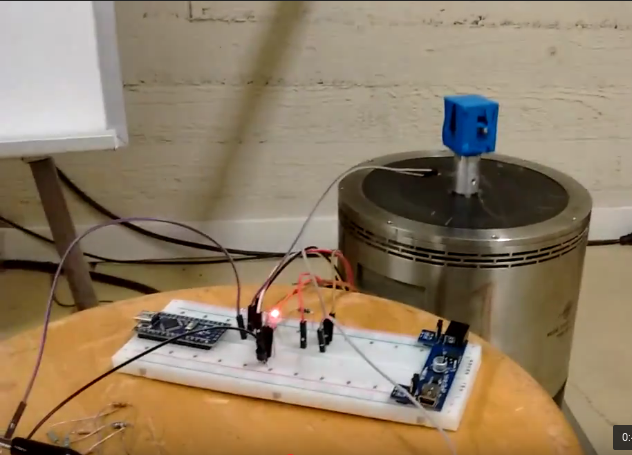
\includegraphics[height=8cm]{images/own_pic/shaker_setup/emh_shaker.png}
\end{center}
\caption{\label{fig:emh_shaker} Test setup for harvester.}
\end{figure}

The vibration exciter is electromagnetically driven platform which translates electrical signal into mechanical movement. Device under test is fastened onto test "head" of vibration exciter, and the acceleration seen by device is then controlled by electrical signal.

The test setup did not have feedback for the position of the harvester, so exact displacement or acceleration of the harvester is unknown. The output signal from the function generator had amplitude of 6 V peak-to-peak and the gain of power amplifier was set to 9.5 in testing.

\subsection{Experimental results of the electromagnetic harvester}
This section presents the experimental results from electromagnetic harvester on vibration exciter. The electromagnetic harvester was tested both on resistive load and while supplying power to a harvester board. 

The harvester was built according to design presented in Section \ref{sect:emh_design}. Figure \ref{fig:emh_final} shows the completed assembly. The rotor magnet can be seen suspended in the middle of assembly, the coil is formed on the upper half of the generator. A magnetic spring is formed by magnets on top and bottom sides of the harvester. 

\begin{figure}[htb]
\begin{center}
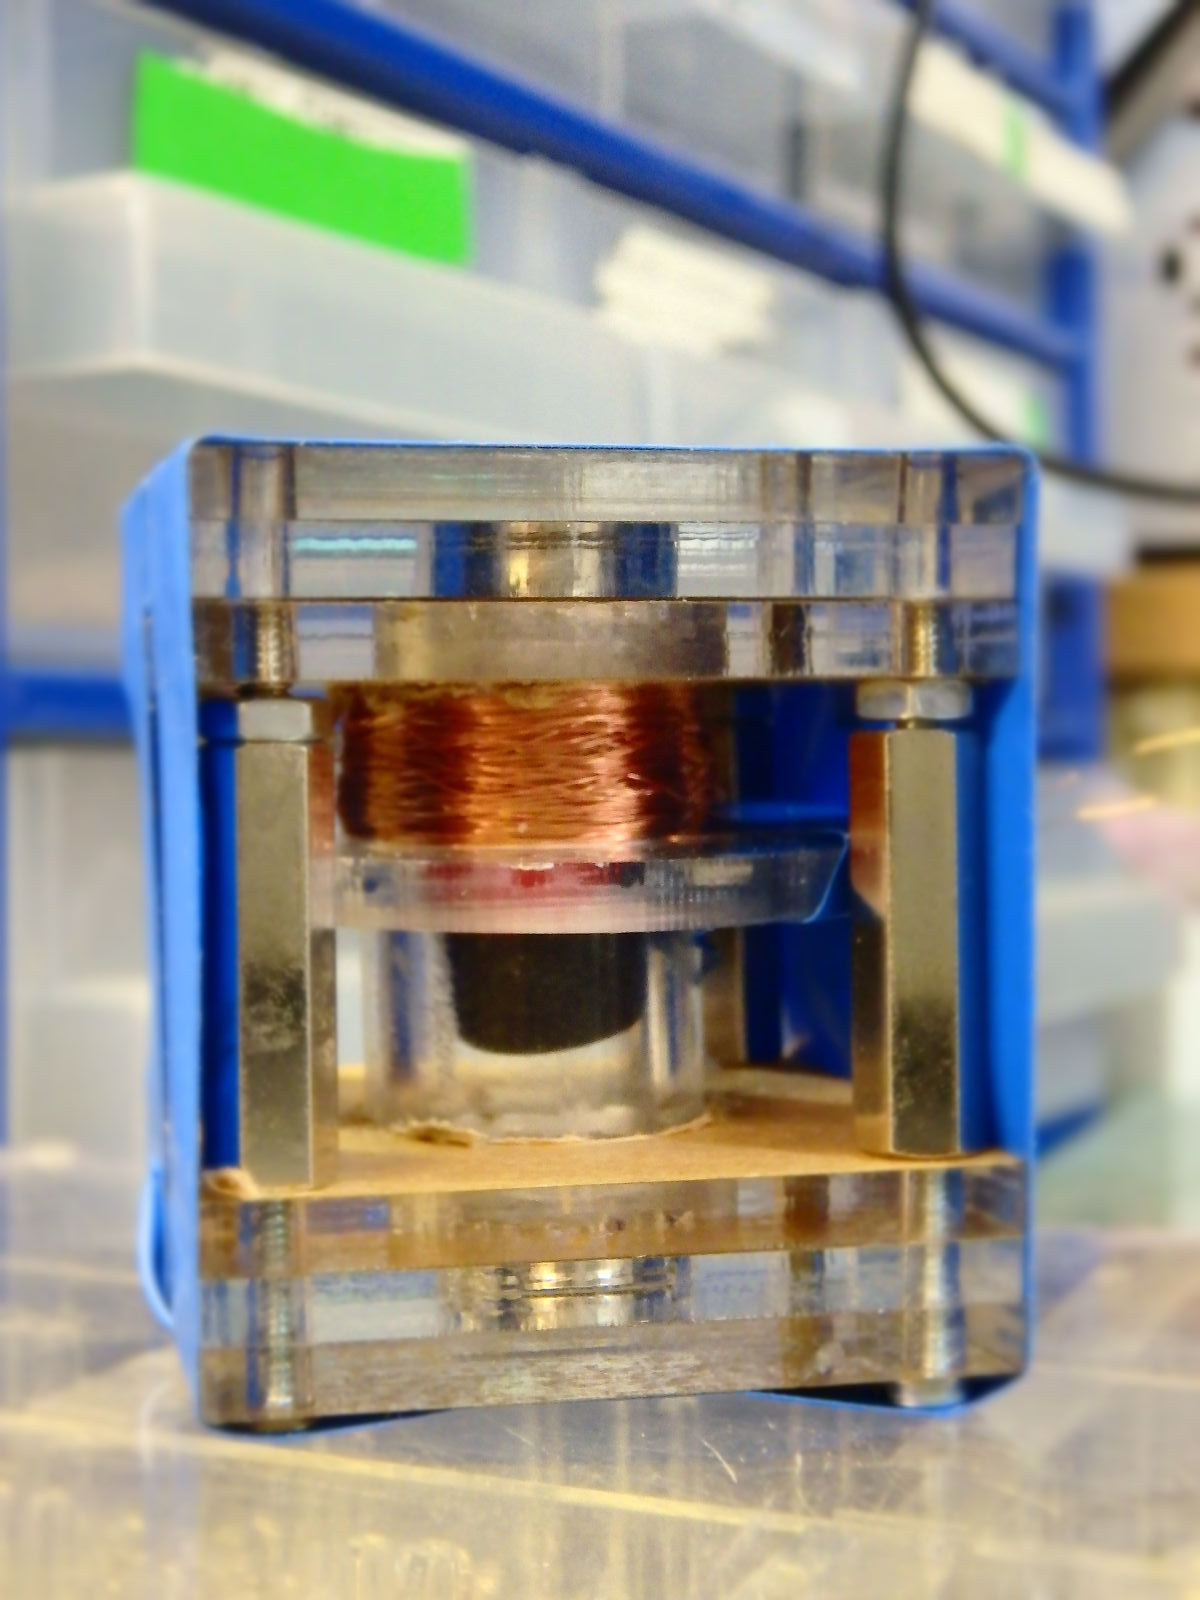
\includegraphics[height=8cm]{images/own_pic/inductive_harvester.jpg}
\end{center}
\caption{\label{fig:emh_final} Final prototype of electromagnetic harvester.}
\end{figure}

\subsubsection{Frequency domain results} \label{sect:emh_fd}
One of the original design goals of the harvester was to provide a wide-band energy harvester solution. This section presents the frequency domain response of the electromagnetic harvester.

Frequency domain response was obtained by sweeping a wide-band sine signal to power amplifier and measuring the open loop response from the harvester. The rotor magnet was stuck in the shaft of harvester at low frequencies, and the power output fell quickly on high frequencies. To solve this problem with friction, ferrofluid was applied to the rotor magnet. Ferrofluid is oil which has magnetic particles suspended in emulsion, these magnetic particles create effectively magnetic oil which stays on contact with the magnet surfaces. This approach has been used before in a ocean wave energy harvester \cite{Cheung2009}.

 After the application of ferrofluid electromagnetic harvester shows a strong resonance peak near 80 Hz as shown in Figure \ref{fig:inductive_fd_dry}. Above graph is the output in decibels, below is the phase shift of the response. Phase shift behaviour was not affected by ferrofluid lubrication. Usually the systems which have second order dynamics - such as the mass damper spring system - exhibit resonance peaks when the damping factor is low. It is can therefore be concluded that application of ferrofluid has resulted in lesser frictional losses. Amplitude response is also at higher level across all frequencies, suggesting a better overall performance of the harvester. 

\begin{figure}[htb]
\begin{center}
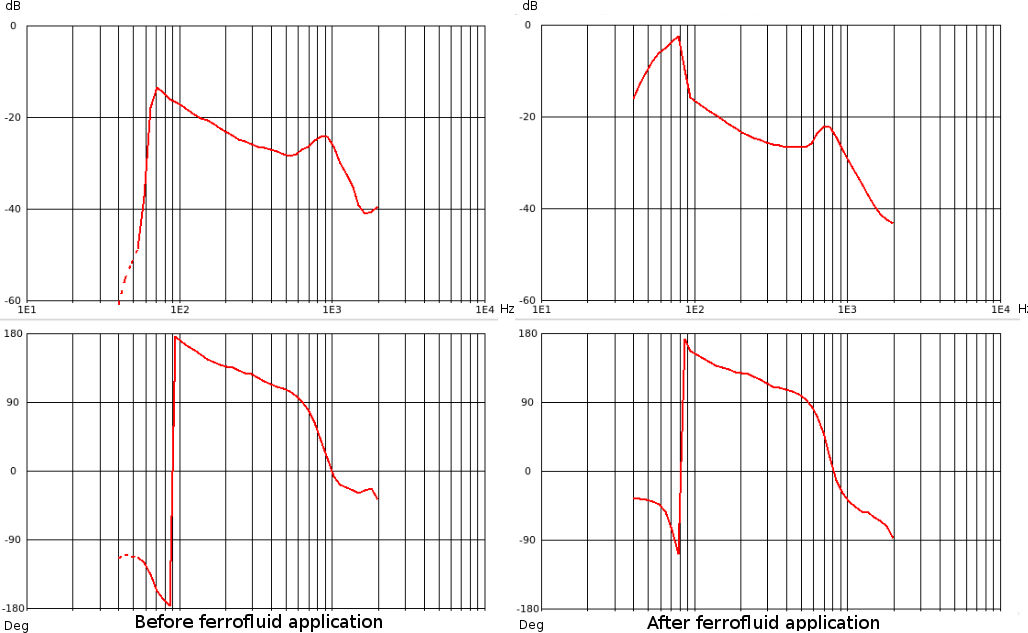
\includegraphics[width=\columnwidth]{images/own_measurement/generator_shaker/inductive_fd_combined.png}
\end{center}
\caption{\label{fig:inductive_fd_dry} Frequency domain response of electromagnetic harvester before and after application of ferrofluid. Above graph is the amplitude response, bottom is the phase shift. After application of ferrofluid the resonance peak is notably sharper, indicating a higher quality factor.  }
\end{figure}

The phase shift is almost exactly 180\degree \ at the resonance, which is somewhat curious result as the time domain results and theory predicted the voltage would peak at 90\degree \ phase when the acceleration is at zero and speed is highest. Amplitude does not have any specific meaning outside the context of this measurement and comparing output at different frequencies.  There is another resonance peak near 900 Hz, but this frequency is far above frequencies of interest for the application. The -3 dB bandwidth is $ \approx $ 10 Hz wide, which can be compared to results of Singh et al. \cite{Singh2012} referred in Section \ref{sect:background}. Singh et al. achieved approximately 5 Hz wide -3 dB bandwidth with piezoelectric harvester 70 Hz.


\subsubsection{Time domain results}\label{sect:lg_td}
The time domain waveforms of the electromagnetic harvester were measured on various loads and frequencies. After the open loop results were obtained, the tests were run again with different resistive loads to measure the power output. Finally the power output to the rectifier of the harvesting circuit of was measured. This section presents the test results. 

The magnet inside the harvester had a notable amount of friction which had to be overcome before any output could be obtained from the harvester. It was not possible to obtain very small signals from harvester, as any input strong enough to move the magnet resulted in a volt-scale output. Figure \ref{fig:inductive_65_open_dry} shows an example of waveforms obtained from harvester. 

\begin{figure}[htb]
\begin{center}
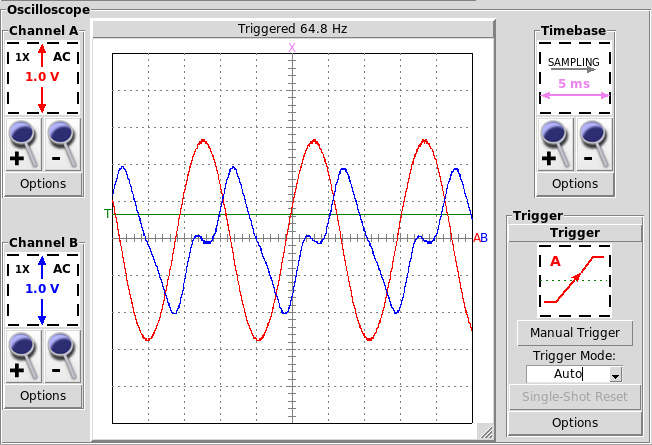
\includegraphics[height=10cm]{images/own_measurement/generator_shaker/inductive_td_open_65hz_dry.png}
\end{center}
\caption{\label{fig:inductive_65_open_dry} Open circuit response of the electromagnetic harvester. Red is the excitation waveform, blue is the open-circuit voltage from the harvester.}
\end{figure}

The waveforms presented in Figure \ref{fig:inductive_65_open_dry} have some curious features: the response from the harvester is asymmetric, there is a notable valley of no output on the rising edge of the signal while no such edge is visible on falling edge. It should be noted that these valleys do not necessarily correspond to the direction of gravity: the phase of input/output signal can be inversed at any point in the signal chain as the polarity of magnet, direction of the winding of coils, and connection of wires can change.

There seems to be a 90\degree \ phase shift between excitation and response. This phase shift was expected, as the excitation signal drives acceleration to exciter, so speed of the magnet reaches maximum at the zero-crossings of excitation. This observation matches well theory presented in Section \ref{sect:em_harvest}: Voltage is proportional to the rate of change of magnetic field. 

Amplitude of output is 2 V and the resistance of the coil was measured to be 34 $\Omega$ at DC. Inductive component of the coil impedance is negligible at the frequencies of interest, so only the resistive component needs to be considered. The Optimal load would then be 34 $\Omega$. When these values are substituted in time domain into Equation \ref{eq:generator_load_power} in Section \ref{sect:em_harvest} we obtain:

\begin{equation}\label{eq:emh_resistive_power_output}
  P_{load}(t) = V(t) \cdot \frac{ 34 \Omega }{ 34 \Omega + 34 \Omega } \cdot \frac{ V(t) }{ 34 \Omega + 34 \Omega } = \frac{V(t)^2}{136 \Omega}
\end{equation}

When peak amplitude of 2 V is inserted to the Equation \eqref{eq:emh_resistive_power_output} peak power is $ \approx 30 mW $. Root mean square (RMS) voltages are used to express the average power over time. RMS cannot be accurately calculated from given values, as the waveform is not  mathematically perfect. If the waveform is approximated as triangle wave, the RMS power would be 

\begin{equation} \label{eq:rms_power}
  P_{rms} = k * P_{peak} = \frac{1}{\sqrt{3}} * 30 mW \approx 17 mW 
\end{equation}
where $k$ is a constant multiplier for RMS power for triangle waves. 
If the excitation power was increased until rotor magnet audibly contacted the endstop magnets, there was no significant change in output voltage. One possible explanation is the valley in output waveform: maybe the rotor magnet was driven to near-contact to stator magnet and when the acceleration was reduced the rotor magnet was accelerated mainly by the magnetic interaction. The end result would be that the length of the valley in the output waveform would vary while the output amplitude would be limited by the magnetic interaction. While further exploration of this phenomenon would be interesting, the testing would be potentially destructive and therefore those experiments were left to future work.

This harvester cannot be used with the circuit designed in Section \ref{sect:electronic_design} as the output amplitude is only 2 V at any reasonable acceleration and frequency. The circuit would require minimum of 4 V to get out of the undervoltage lockout, and this is not achievable even by connecting the bridge rectifier as a voltage doubler because the energy harvesting input still has two diode drops which would keep the voltage below the required threshold.

Next test was done by connecting the harvester to a boost circuit based on TI BQ25504 \cite{bq25504}. BQ25504 has a boost-mode SMPS in energy harvesting input which is able to utilise input voltages as low as 80 mV after startup and it can start up at roughly 330 mV. The detailed description of the circuit is given in Section \ref{sect:BQ25504_schematic}. The issue with diode voltage drops was remedied by using schottcky-diodes connected as voltage doubler.

To measure the actual power output, a current-to-voltage converter $\mu$Current \cite{Jones2010} was connected in series to the output of harvester. Measurement was done at scale 1 V = 1 mA. Waveforms are shown in figure \ref{fig:inductive_vi_65}. It should be noted that the current channel might be saturated, as the $\mu$Current cannot produce output higher than 1.25 V.

\begin{figure}[htb]
\begin{center}
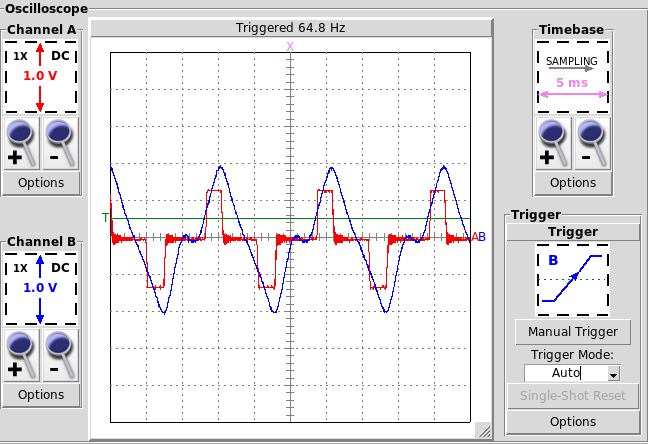
\includegraphics[height=10cm]{images/own_measurement/generator_shaker/inductive_td_harvesting_vi_65hz_ferro.png}
\end{center}
\caption{\label{fig:inductive_vi_65} Voltage and current waveform from harvester. Red is current, 1 V equals 1 mA. Blue is voltage from the terminals of harvester before rectification.}
\end{figure}

The waveforms are as expected, there is no current flowing while the voltage is low. When the voltage rises to roughly one volt, current starts to flow charging the output capacitor. When the input voltage starts to decrease, no more current flows to the capacitor. Accuracy of amplitude of current measurement is questionable because of potential saturation of the measuring instrument.

It is worth noting that the voltage rises to open-loop maximum amplitude of 2 V as the loading on the harvester decreases as the voltage on capacitor increases. This indicates that maximum theoretical peak power output of $\approx$ 30 mW is not reached at any point. 

Power waveform of the harvester is presented in Figure \ref{fig:inductive_power_65}. The waveform is calculated by multiplying the voltage and current. Because the current is scaled at 1 mA = 1 V, the result can be read as 1 V = 1 mW. While absolute value of power is questionable because of the potentially saturated instrument, the waveform itself is correct.  

\begin{figure}[htb]
\begin{center}
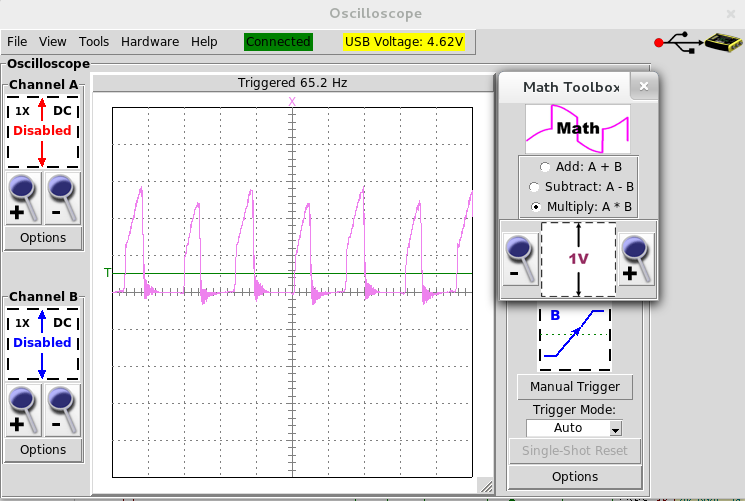
\includegraphics[height=10cm]{images/own_measurement/generator_shaker/inductive_td_harvesting_power_65Hz_ferro.png}
\end{center}
\caption{\label{fig:inductive_power_65} Power waveform from harvester. Pink is power, 1 V equals 1 mW.}
\end{figure}

Graphically read average power output is 0.375 mW. One possible reason for the greatly lower power output was the capacitors in voltage doubler structure: the voltage doubler has series capacitance of 10 $\mu$F, which has a reactive impedance of

\begin{equation}
  X_c = \frac{1}{2 \pi f C}  = \frac{1}{2 \pi 65 10\mu} \approx 245 \Omega
\end{equation}
at 65 Hz. Total output impedance of circuit would be approximately 280 $\Omega$, which would limit the output current to approximately 7 mA. This theory was tested by simulating the equivalent model of input section of harvester circuit. Simulation model and results are shown in Figure \ref{fig:simulated_doubler}.

\begin{figure}[htb]
\begin{center}
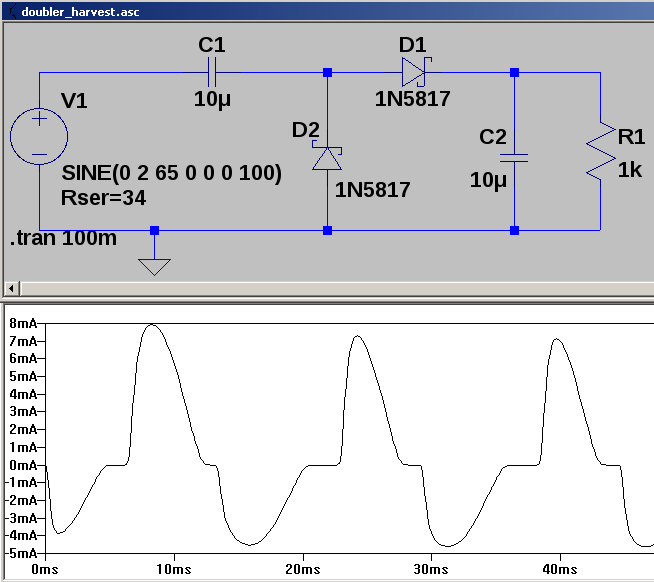
\includegraphics[height=10cm]{images/own_dwg/simulation/voltage_doubler.png}
\end{center}
\caption{\label{fig:simulated_doubler} LTSpice model of energy harvester input section.}
\end{figure}

The simulated data confirms the effect of input capacitor to current output of the system. Current is limited to roughly 7 mA. Simulated power output was on average 2.0 mW. If the measured current is assumed to be limited by saturation, and if we assume that simulated current of 8 mA peaks would be correct, the calculated power output from experimental result would be 

\begin{equation}
\begin{split}
  P_{true}& = P_{simulated} * \frac{I_{simulated}}{I_{real}} \\
  P_{true}& = 0.375 * \frac{7}{1.25} \\
  P_{true}& = 2.1 mW. \\
\end{split}
\end{equation}

After correcting the experimental current with the simulated value, a lot more reasonable value of approximately 2 mW of generated power is obtained. 

This section presented the time-domain results of the electromagnetic harvester on a vibration exciter test platform. Approximately 30 mW peak power was obtained, RMS power of 17 mW was achieved to resistive load and power output to harvester was determined to be in range between 0.4 mW and 2 mW. 

\subsection{Experimental results of the piezoelectric harvester}
\subsubsection{Frequency domain results} \label{sect:piezo_fd}
The frequency domain response of the piezoelectric harvester was obtained in similar manner as with the electromagnetic harvester detailed in Section \ref{sect:emh_fd}. The excitation signal was swept across a wide spectrum and output from the harvester was measured. Frequency domain results are presented in this section.

The frequency sweep result on open circuit is shown in Figure \ref{fig:piezo_fd}. A resonance peak can be found at 334 Hz. Similarly to the electromagnetic harvester, the slope is a lot steeper on the frequencies above the resonance peak than below. 

\begin{figure}[htb]
\begin{center}
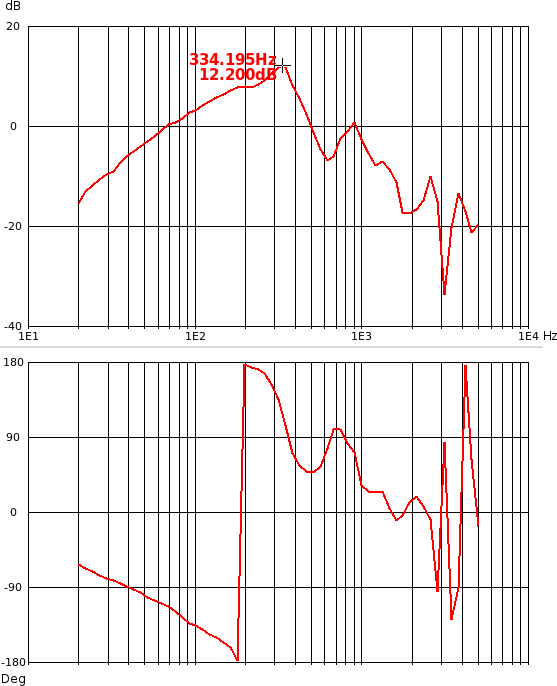
\includegraphics[height=10cm]{images/own_measurement/generator_shaker/piezo_fd_open_2_3.png}
\end{center}
\caption{\label{fig:piezo_fd} Frequency response of piezoelectric harvester}
\end{figure}


The peak frequency is somewhat poorly suited to the environment in the tyre presented in Section \ref{sect:tyre_environment}, as the peak response is significantly above peak frequencies encountered in the tyre. Usually the frequency is tuned downwards by adding mass to the harvester, however this approach is not feasible in this application as the proof mass is limited to avoid damage to the piezoelement due to excessive strain. As the peak frequency was identified near 330 Hz, the time domain analysis were performed on the harvester. Next section details the voltage, current and power outputs into varied loads.

\subsubsection{Time domain results}\label{sect:piezo_td}
This section presents the time-domain results of the piezoelectric harvester. The test setup of the piezoelectric harvester was similar to the test setup of the electromagnetic harvester, details of the test setup are given in Section \ref{sect:lg_test_setup}. Unlike the electromagnetic harvester, this piezoelectric harvester did not have any obvious minimum acceleration before the friction would be overcome and therefore even very small signal was obtainable. Likewise no maximum value for output signal was found by increasing the power to the vibration exciter. The function generator output signal was held at 6 volts peak-to-peak for the time domain tests and at 3 volts peak-to-peak for frequency domain tests to limit the loosening of the screws by vibration. Gain of the power amplifier was fixed at 9.5.

The piezoelectric harvester was characterised by high output voltages at high output impedance. Open loop response is shown in Figure \ref{fig:piezo_td_open}. The output was not a clean sine-resembling signal as with the electromagnetic harvester, it has sharp downwards peaks and a lot of high-frequency distortion.

\begin{figure}[htb]
\begin{center}
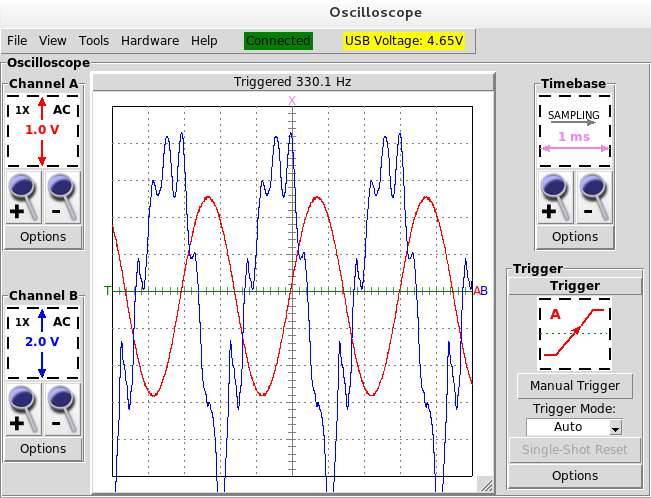
\includegraphics[height=10cm]{images/own_measurement/generator_shaker/piezo_td_open_330hz_2_2.png}
\end{center}
\caption{\label{fig:piezo_td_open} Open loop response from the piezoelectric harvester. Red is the excitation signal, blue is the response.}
\end{figure}

While output signal is off the scale, negative peaks were measured at -12 V. Peak-to-peak amplitude was therefore roughly 20 V. The search for the maximum power point was started by modeling the circuit as RC- high pass filter shown in Figure \ref{fig:rc_highpass} with piezo capacitance as the series capacitor and load as the resistor. 

\begin{figure}[htb]
\begin{center}
\includegraphics[height=4cm]{images/cited/hyperphysics.jpg}
\end{center}
\caption{\label{fig:rc_highpass} RC high pass filter \cite{hyperphysics}.}
\end{figure}

The frequency domain results presented in Section \ref{sect:piezo_fd} were used to find the maximum output frequency at 330 Hz. This frequency was taken as the target cut-off frequency for the RC-filter equation:

\begin{equation}
\begin{split}
  F_c &= \frac{1}{2 \pi R C} \\
  R   &= \frac{1}{2 \pi C F}  = \frac{1}{2 \pi 39 nF 330 Hz} \approx 12 400 \Omega 
\end{split}
\end{equation}

Theory would predict the maximum power point to be near the cut-off frequency, so the generator was tested with 18k$\Omega$, 12k$\Omega$ and 9k$\Omega$ resistive loads. The peak voltages and calculated power into the load are presented in Table \ref{tbl:piezo_harvester_shaker_output}. The power is calculated by approximating the waveform as a clean sine calculating RMS power from peak voltage values. Method is similar to Equation \eqref{eq:rms_power} presented in Section \ref{sect:lg_td}, but the multiplier $k$ is $\sqrt{2}$ instead of $\sqrt{3}$ as the waveform is approximated as a sine rather than a triangle. While the absolute value of the power output has approximation error, the waveforms obtained with 18 k$\Omega$ and 12 k$\Omega$ are similar enough for comparing the outputs between the loads. On 9 k$\Omega$ load the waveform was clearly more distorted, and therefore calculation for power has greater approximation error.

\begin{table}[htb]
\caption{\label{tbl:piezo_harvester_shaker_output} Output power of piezo harvester at 18 k$\Omega$, 12 k$\Omega$ and 9 k$\Omega$ loads.}
\begin{center}
\fbox{
\begin{tabular}{r l l}
\textbf{Load}          & \textbf{Amplitude} 		& \textbf{Power\textsubscript{rms}}	\\ \hline
18 k$\Omega$  & 7 volts	& 1.36 mW \\ 
12 k$\Omega$  & 6 volts	& 1.50 mW \\ 
9 k $\Omega$  & 4 volts 	& 0.89 mW
\end{tabular}
}
\end{center}
\end{table}

The waveforms from 12 k$\Omega$ load and 9 k$\Omega$ load are shown in Figures \ref{fig:piezo_td_12k} and \ref{fig:piezo_td_9k} for comparing the amount of distortion. While both waveforms show a clear high-frequency content, possibly caused by resonant frequency of piezo element itself, the heavier loading causes a significant distortion on the waveform.

\begin{figure}[htb]
\begin{center}
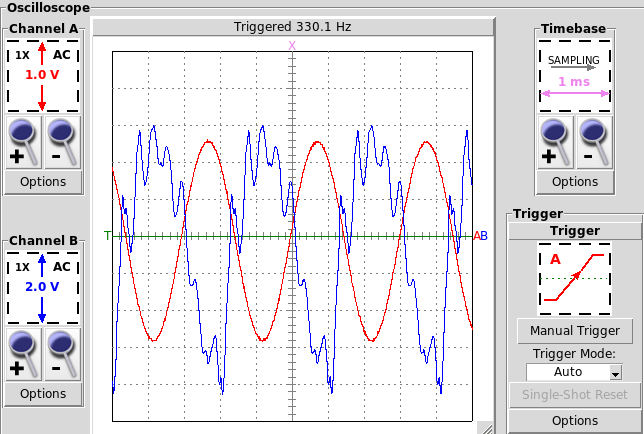
\includegraphics[height=10cm]{images/own_measurement/generator_shaker/piezo_td_12k_330hz_2_2.png}
\end{center}
\caption{\label{fig:piezo_td_12k} Piezoelectric harvester under 12 k$\Omega$ load. Red is the excitation signal, blue is the response.}
\end{figure}

\begin{figure}[htb]
\begin{center}
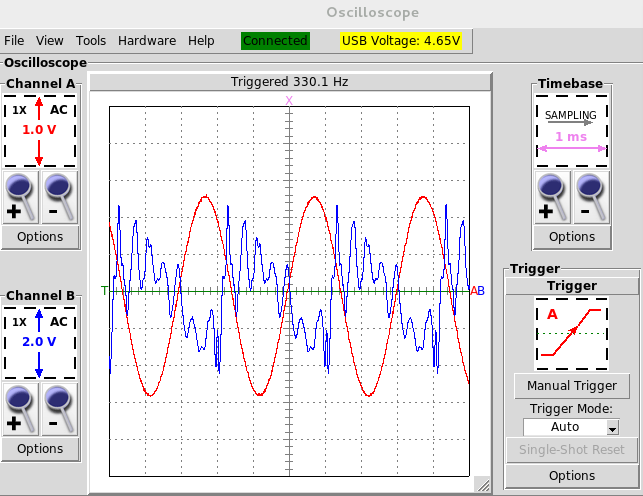
\includegraphics[height=10cm]{images/own_measurement/generator_shaker/piezo_td_9k_330hz_2_2.png}
\end{center}
\caption{\label{fig:piezo_td_9k} Piezoelectric harvester under 9 k$\Omega$ load. Red is excitation signal, blue is response.}
\end{figure}

The waveform on Figure \ref{fig:piezo_td_9k} resembles almost a saw-tooth wave. Regardless of actual RMS value, it can be confidently said that the power output is smaller under 9 k$\Omega$ load than under 12 k$\Omega$ load. Therefore maximum power point can be concluded to be near 12 k$\Omega$ load at 330 Hz. 

After testing the behaviour of piezoelectric harvester on resistive loads, power output to the harvester through rectification was tested. While the electromagnetic harvester had a notably higher output to resistive load, rectification drops voltage and therefore high-voltage characteristic of piezoelectric harvester is advantageous for rectification. 

As with the electromagnetic harvester, current was measured using $\mu$Current at 1 mV / $\mu$A setting. While the electromagnetic harvester suffered from reactance of series capacitance limiting the output of the harvester, output impedance of piezoelectric harvester is a lot higher than impedance of additional series capacitor and therefore the output was not impaired by the coupling capacitance. The VI-waveforms are shown in Figure \ref{fig:piezo_td_vi}. 

\begin{figure}[htb]
\begin{center}
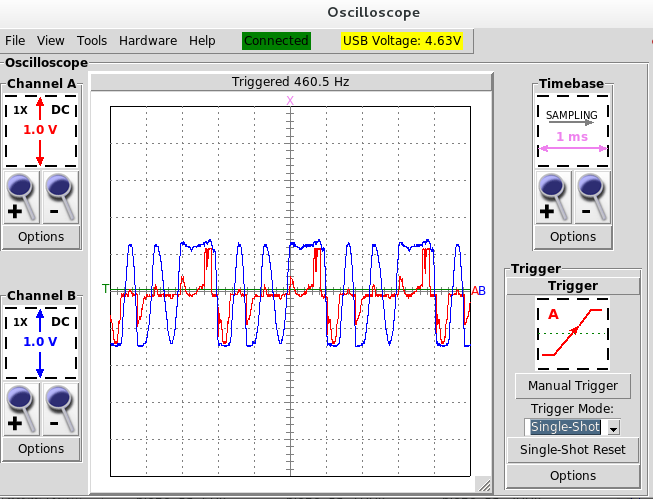
\includegraphics[height=10cm]{images/own_measurement/generator_shaker/piezo_td_vi_330hz_2_3.png}
\end{center}
\caption{\label{fig:piezo_td_vi} VI-waveforms of piezoelectric harvester into rectifier. Blue is voltage, red is current with scaling of 1 mA / V. Current does not follow the voltage and voltage is clamped by diodes.}
\end{figure}

Output of the piezoelectric harvester does not follow the excitation in a similar manner to the electromagnetic harvester. The output voltage is clamped by the diodes of rectification circuit, and the current waveform does not follow the voltage waveform. Power output waveforms have been presented in Figure \ref{fig:piezo_td_power}. As before, the output can be read as 1 V = 1 mW. 

\begin{figure}[htb]
\begin{center}
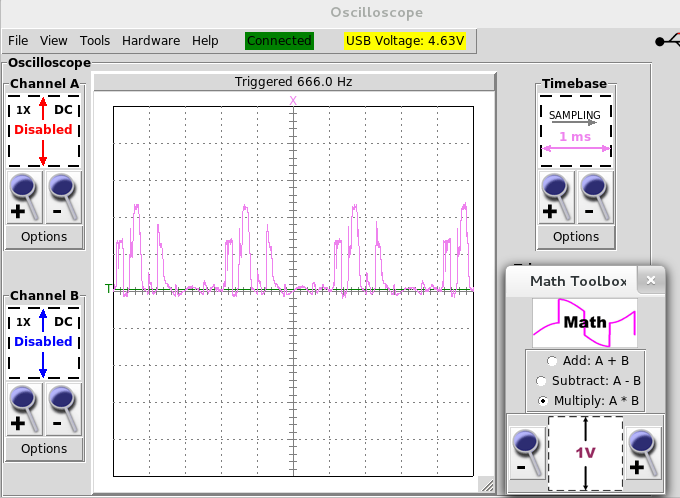
\includegraphics[height=10cm]{images/own_measurement/generator_shaker/piezo_td_power_330hz_2_3.png}
\end{center}
\caption{\label{fig:piezo_td_power} Power waveform of piezoelectric harvester. Scaling is 1 mW / V.}
\end{figure}

While excitation frequency of 330 Hz was not clearly visible in VI-waveforms, the rectified signal is clearly double of 330 Hz. Graphic integration suggests the power output to be in order of hundreds of microwatts, with peak power output being approximately 2.4 mW. 

It can be concluded that piezoelectric harvester produces most of the power at the excitation frequency, any output from the internal resonances are negligible in comparison to energy obtained from the external actuation.

\subsection{Harvesting circuit results}
\subsubsection{Revisited circuit design}\label{sect:BQ25504_schematic}
While the original idea was to use the circuit presented in Section \ref{sect:electronic_design} for testing the system-level performance, it became obvious that the harvesters cannot produce output levels required by the circuit. A new simplified harvesting circuit was designed to test the performance of the harvester inside the tyre. The harvester design is presented in this section.

According to Rouvala, M. \cite{Rouvala2015} best way to utilise low output levels is to chain voltage multiplier circuit stages to produce higher DC-level and then use a boost circuit to bring the harvested output into desired level. A few ICs from different manufacturers were considered for the new circuit, namely Seiko S-882z \cite{SeikoInstruments2010} charge pumps, Linear Technology LTC3105 \cite{ltc3015} boost charger and Texas Instruments BQ255xx -series boost chargers. As Seiko ICs are not readily available and LTC3105 requires high start-up currents, BQ25504 \cite{bq25504} was chosen as the core for the harvesting circuit. The schematic of harvesting circuit is presented in Figure \ref{fig:bq25504} and Figure \ref{fig:bq25504_mounted} shows the assembled circuit mounted on top of the piezoelectric harvester.


\begin{figure}[htb]
    \centering
    \def\svgwidth{\columnwidth}
    \input{images/own_dwg/circuit/bq25504.pdf_tex}
    \caption{\label{fig:bq25504} Schematic of the revised harvester circuit. Inputs are to left, both AC and DC input is supported. Resistors R1 and R2 set the maximum power point tracking point. Resistors R3 ... R9 set operation points: such as target voltage as 3.3 V, power good thresholds and undervoltage lockout threshold at 2.2 V. C5 is the supercapacitor for storing energy, C7 is a ceramic capacitor for rejecting high-frequency noise. C3 provides high-frequency filtering for switched power supply noise and C4 is bulk capacitance for load. Over Temperature shutdown treshold (OT\_PROG) is set to 120 $\degree$C by pulling OT\_PROG to a high voltage level. VBAT\_OK signal is a digital output which can be used to wake sensor platform when enough energy has been stored for taking a measurement and transmitting data.}
\end{figure}

\begin{figure}[htb]
\begin{center}
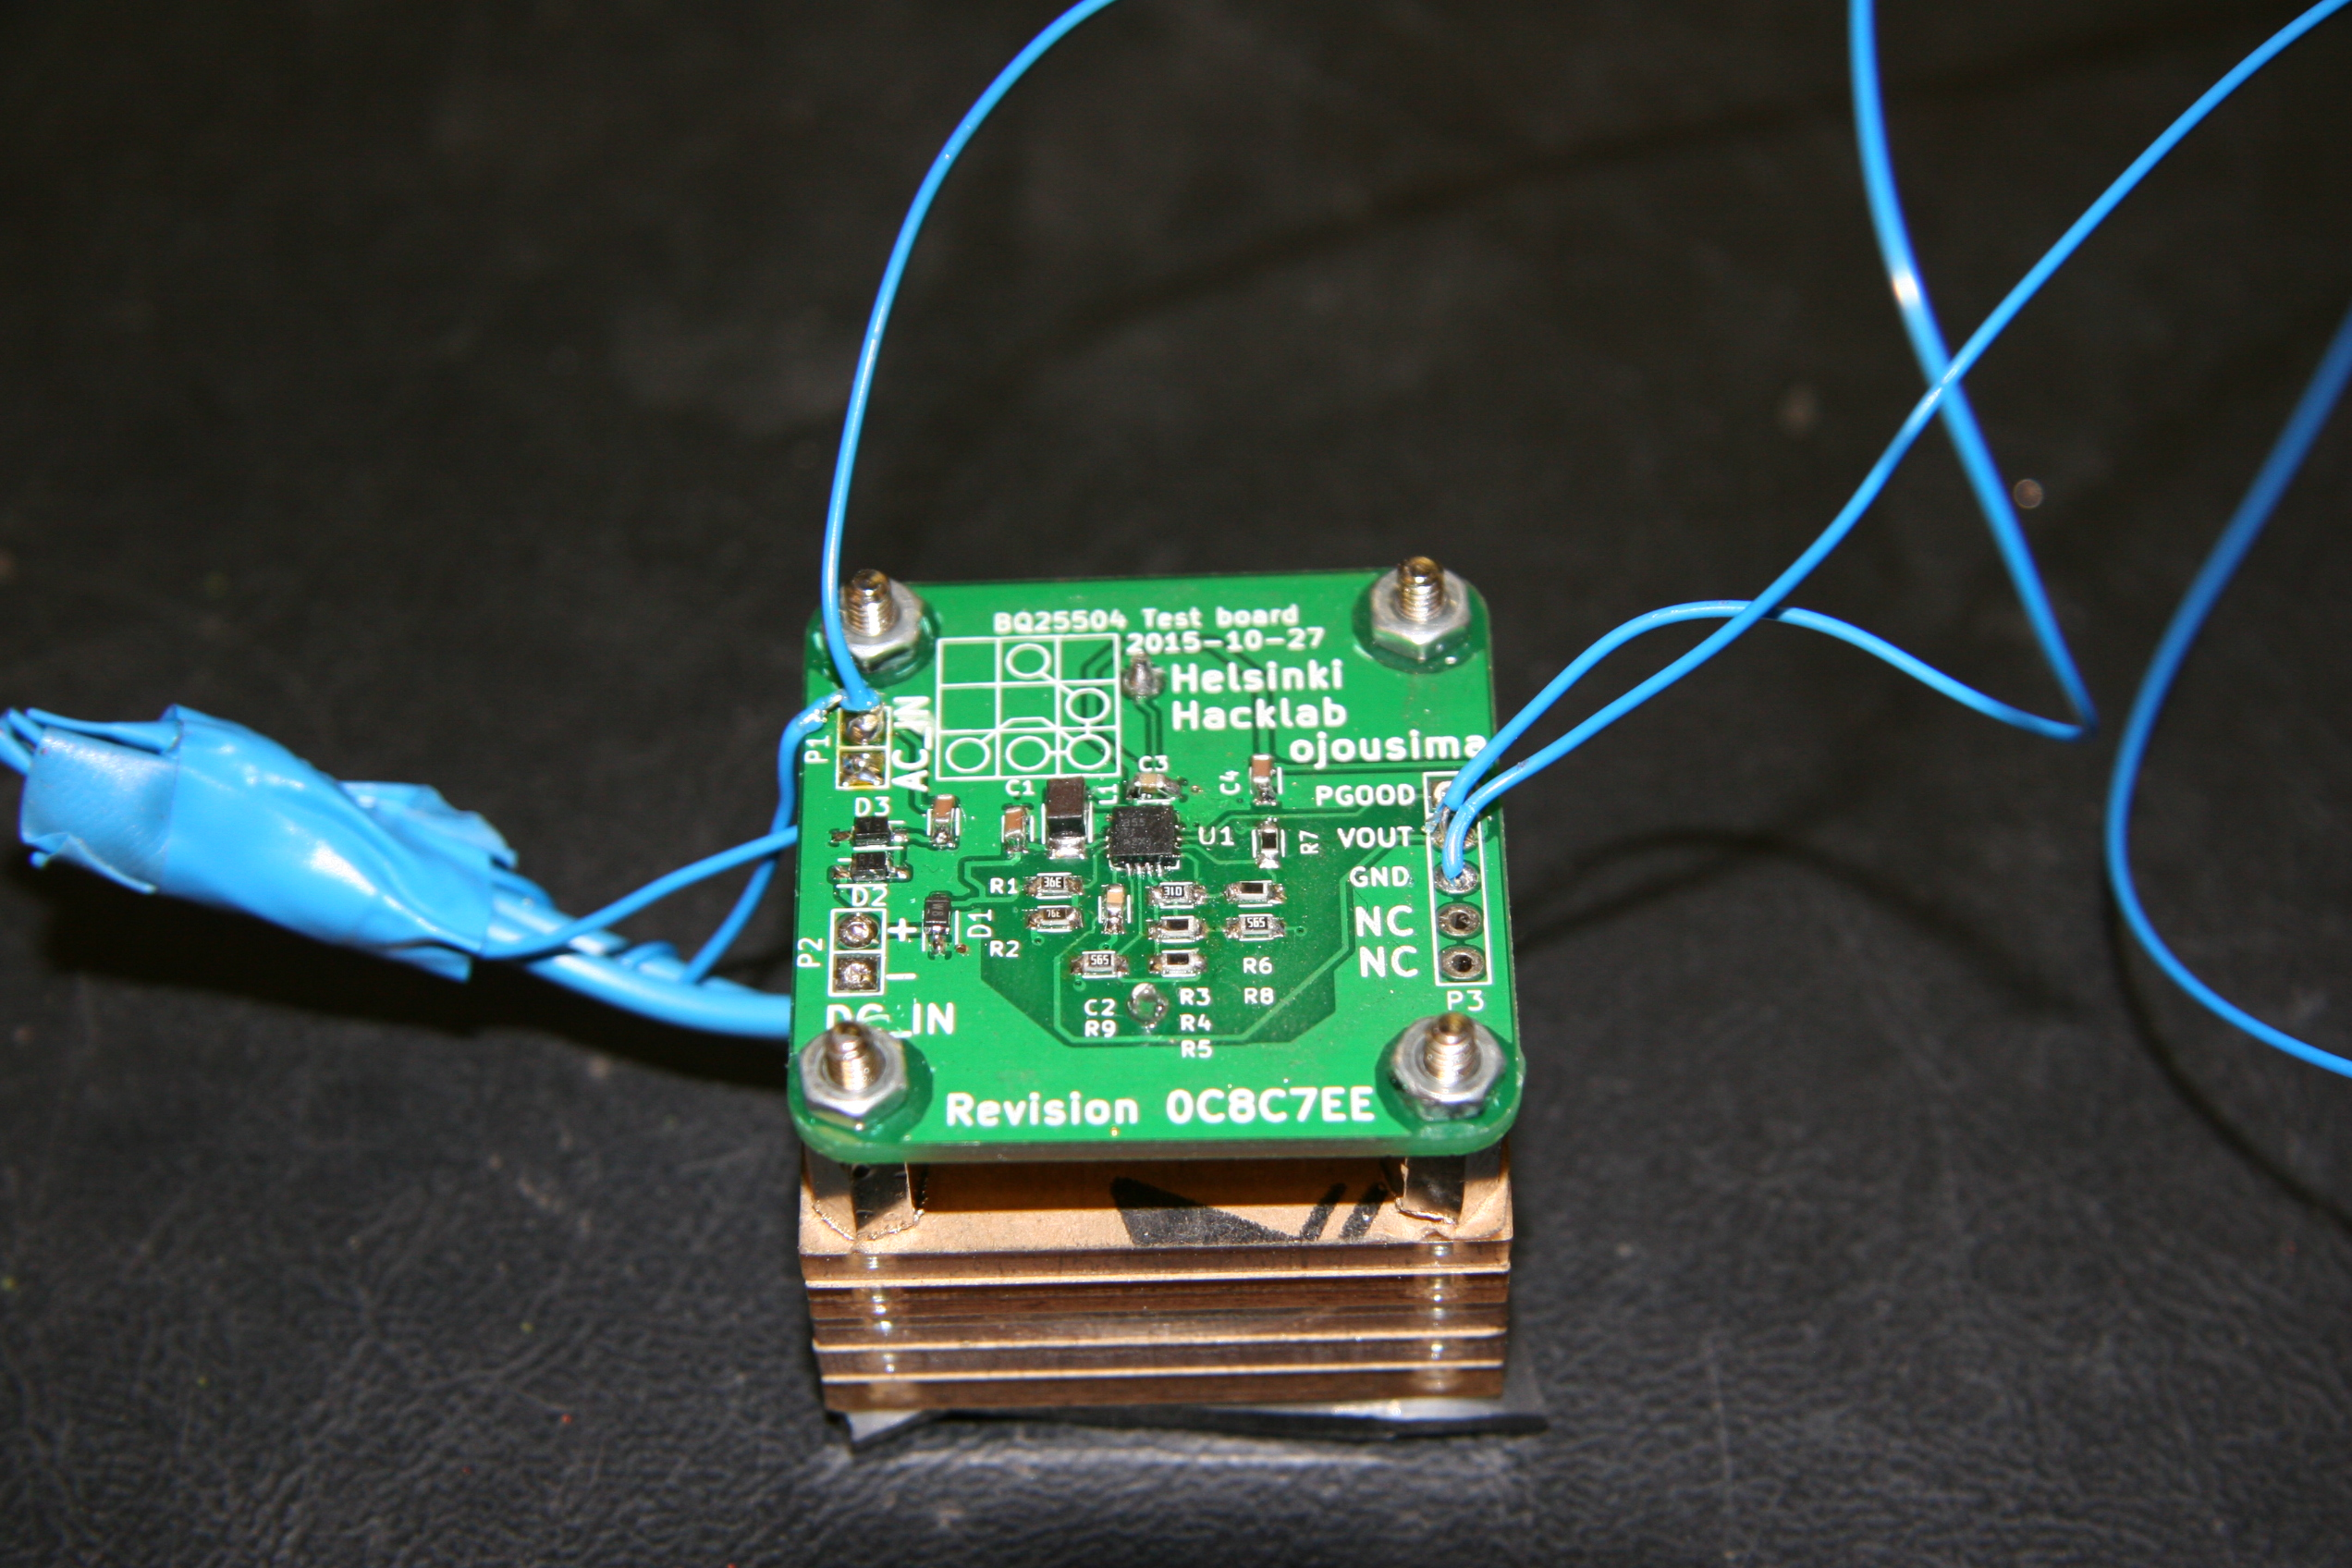
\includegraphics[height=8cm]{images/own_pic/tyre_fixture/piezo_bq_desk.jpg}
\end{center}
\caption{\label{fig:bq25504_mounted} BQ25504-based harvesting circuit mounted on piezoelectric harvester.}
\end{figure}

The revised harvesting circuit is able to start at 0.33 V input DC voltage, or at near 0.4 V RMS amplitude AC voltage contrasted to 5 V DC level of LTC3331-based circuit. A supercapacitor was chosen as energy storage for easy measurement of accumulated harvested energy. The supercapacitor was model EECRG0V155VN \cite{panasonic_scap} with 3.6 V maximum voltage and 1.5 F nominal capacitance. 

Maximum power point tracking is provided by sampling open-loop voltage of the circuit through voltage divider R1 and R2 every 16 seconds into capacitor C2. After the sample has been stored into the capacitor, BQ25504 attempts to set the current taken from the input so that V\textsubscript{IN} matches V\textsubscript{REF}. 

This form of MPPT is not adjustable by an external microcontroller: while digital potentiometers exist, their current consumption far exceeds the low-power requirements of the circuit. Therefore a fixed ratio had to be set for the circuit. The ratio was set to 80 \% to avoid overloading the piezoelement, as it was previously found in section \ref{sect:piezo_td} that overloading the element has a disastrous effect on efficiency of piezoelectric harvesting whereas underloading has much less pronounced effect on the efficiency.

Resistors R3 through R9 set various operation points for the circuit. Output voltage was set to 3.3 V, and power good -threshold was set to 3 V on charging and 2.2 V on discharging. 

The circuit was built and found to work with both harvester designs on the vibration exciter. As the circuit was usable, further work was carried out using this circuit. Next section details the measurement of the supercapacitor parameters after it was soldered in the circuit.

\subsubsection{Measuring the supercapacitor parameters}
As the energy storage used in the circuit is a supercapacitor and all subsequent measurements are based on values measured from the supercapacitor, the supercapacitor was characterised in-circuit to obtain more accurate values for the system performance. The measuring process and the results are presented in this section.

Application note AN1005 from Cap-XX \cite{an1005} details a simple process for measuring supercapacitor capacitance and Equivalent Series Resistance (ESR). The supercapacitor is first charged to a target voltage and then discharged through a resistor. The parameters are then read from the discharge waveform. A 100 ohm resistor was used as the discharging resistance, the discharge waveform is shown in Figure \ref{fig:scap_discharge}. 

\begin{figure}[htb]
\begin{center}
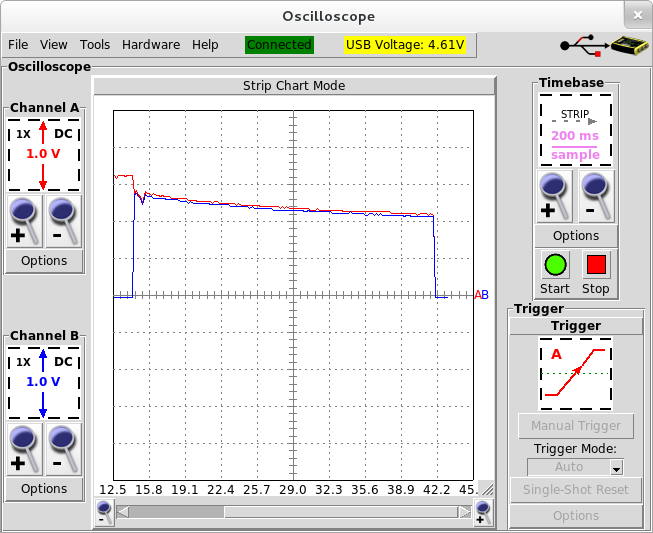
\includegraphics[height=8cm]{images/own_measurement/circuit/discharge.png}
\end{center}
\caption{\label{fig:scap_discharge} Discharge waveform. Red is the capacitor voltage, blue is voltage over 100 ohm resistor.}
\end{figure}

The initial discharge current can be calculated with voltage over resistor:

\begin{equation}
  I_{initial} = \frac{V_{initial}}{R} = \frac{2.75 V}{100 \Omega} \approx 27.5 mA 
\end{equation}

With the initial discharge current and voltage drop known, ESR can be calculated:

\begin{equation}
  ESR = \frac{V_{0} - V_{initial}}{I_{initial}} = \frac{3.25 V - 2.75 V}{27.5 mA} \approx 18.2 \Omega
\end{equation}

With ESR known, it is possible to calculate capacitance from the discharge time:

\begin{equation}
\begin{split}
  V_t                            &= V_{initial}e^{-t/R_{tot}C} \\
  \frac{V_t}{V_{initial}}                &= e^{-t/R_{tot}C} \\
  ln\left(\frac{V_t}{V_{initial}}\right) &= \frac{-t}{R_{tot}C} \\
  C                              &= \frac{-t}{R_{tot}} \frac{1}{ ln\left(\frac{V_t}{V_{initial}}\right)} = \frac{41.6-14.4}{100 + 18.2} \frac{1}{ ln\left(\frac{2.75 V}{3.25 V}\right)} &\approx 1.38 F
\end{split}
\end{equation}

Therefore the capacitor ESR was found to be 18.2 $\Omega$ and capacitance 1.37 F. This is well within the published initial values of ESR < 30 $\Omega$ and capacitance of 1.5 F -20 \% ... + 80 \%, and therefore the results can be considered reliable. 

As the devices were proven in a laboratory setting, further test was carried out to determine the power output in a simulated drive inside a tyre. The test setup and results are detailed in next section.

\subsection{Performance inside tyre}
The final experiment was to install the piezoelectric harvester with revisited electronics inside the tyre and simulate driving conditions with a dynamometer platform. Piezoelectric harvester was chosen for the final tests as it was able to produce output even with small excitation unlike electromagnetic harvester which required a minimum impact before producing power. The test results are presented in this section. 

The harvester was glued to the inner lining of the tyre as shown in Figure \ref{fig:harvester_potted} and electrical connections were brought through a slip ring for instrumentation. The tyre was installed to rig presented in Figure \ref{fig:tyre_platform} and the tyre was driven at various speeds and loads. 

\begin{figure}[htb]
\begin{center}
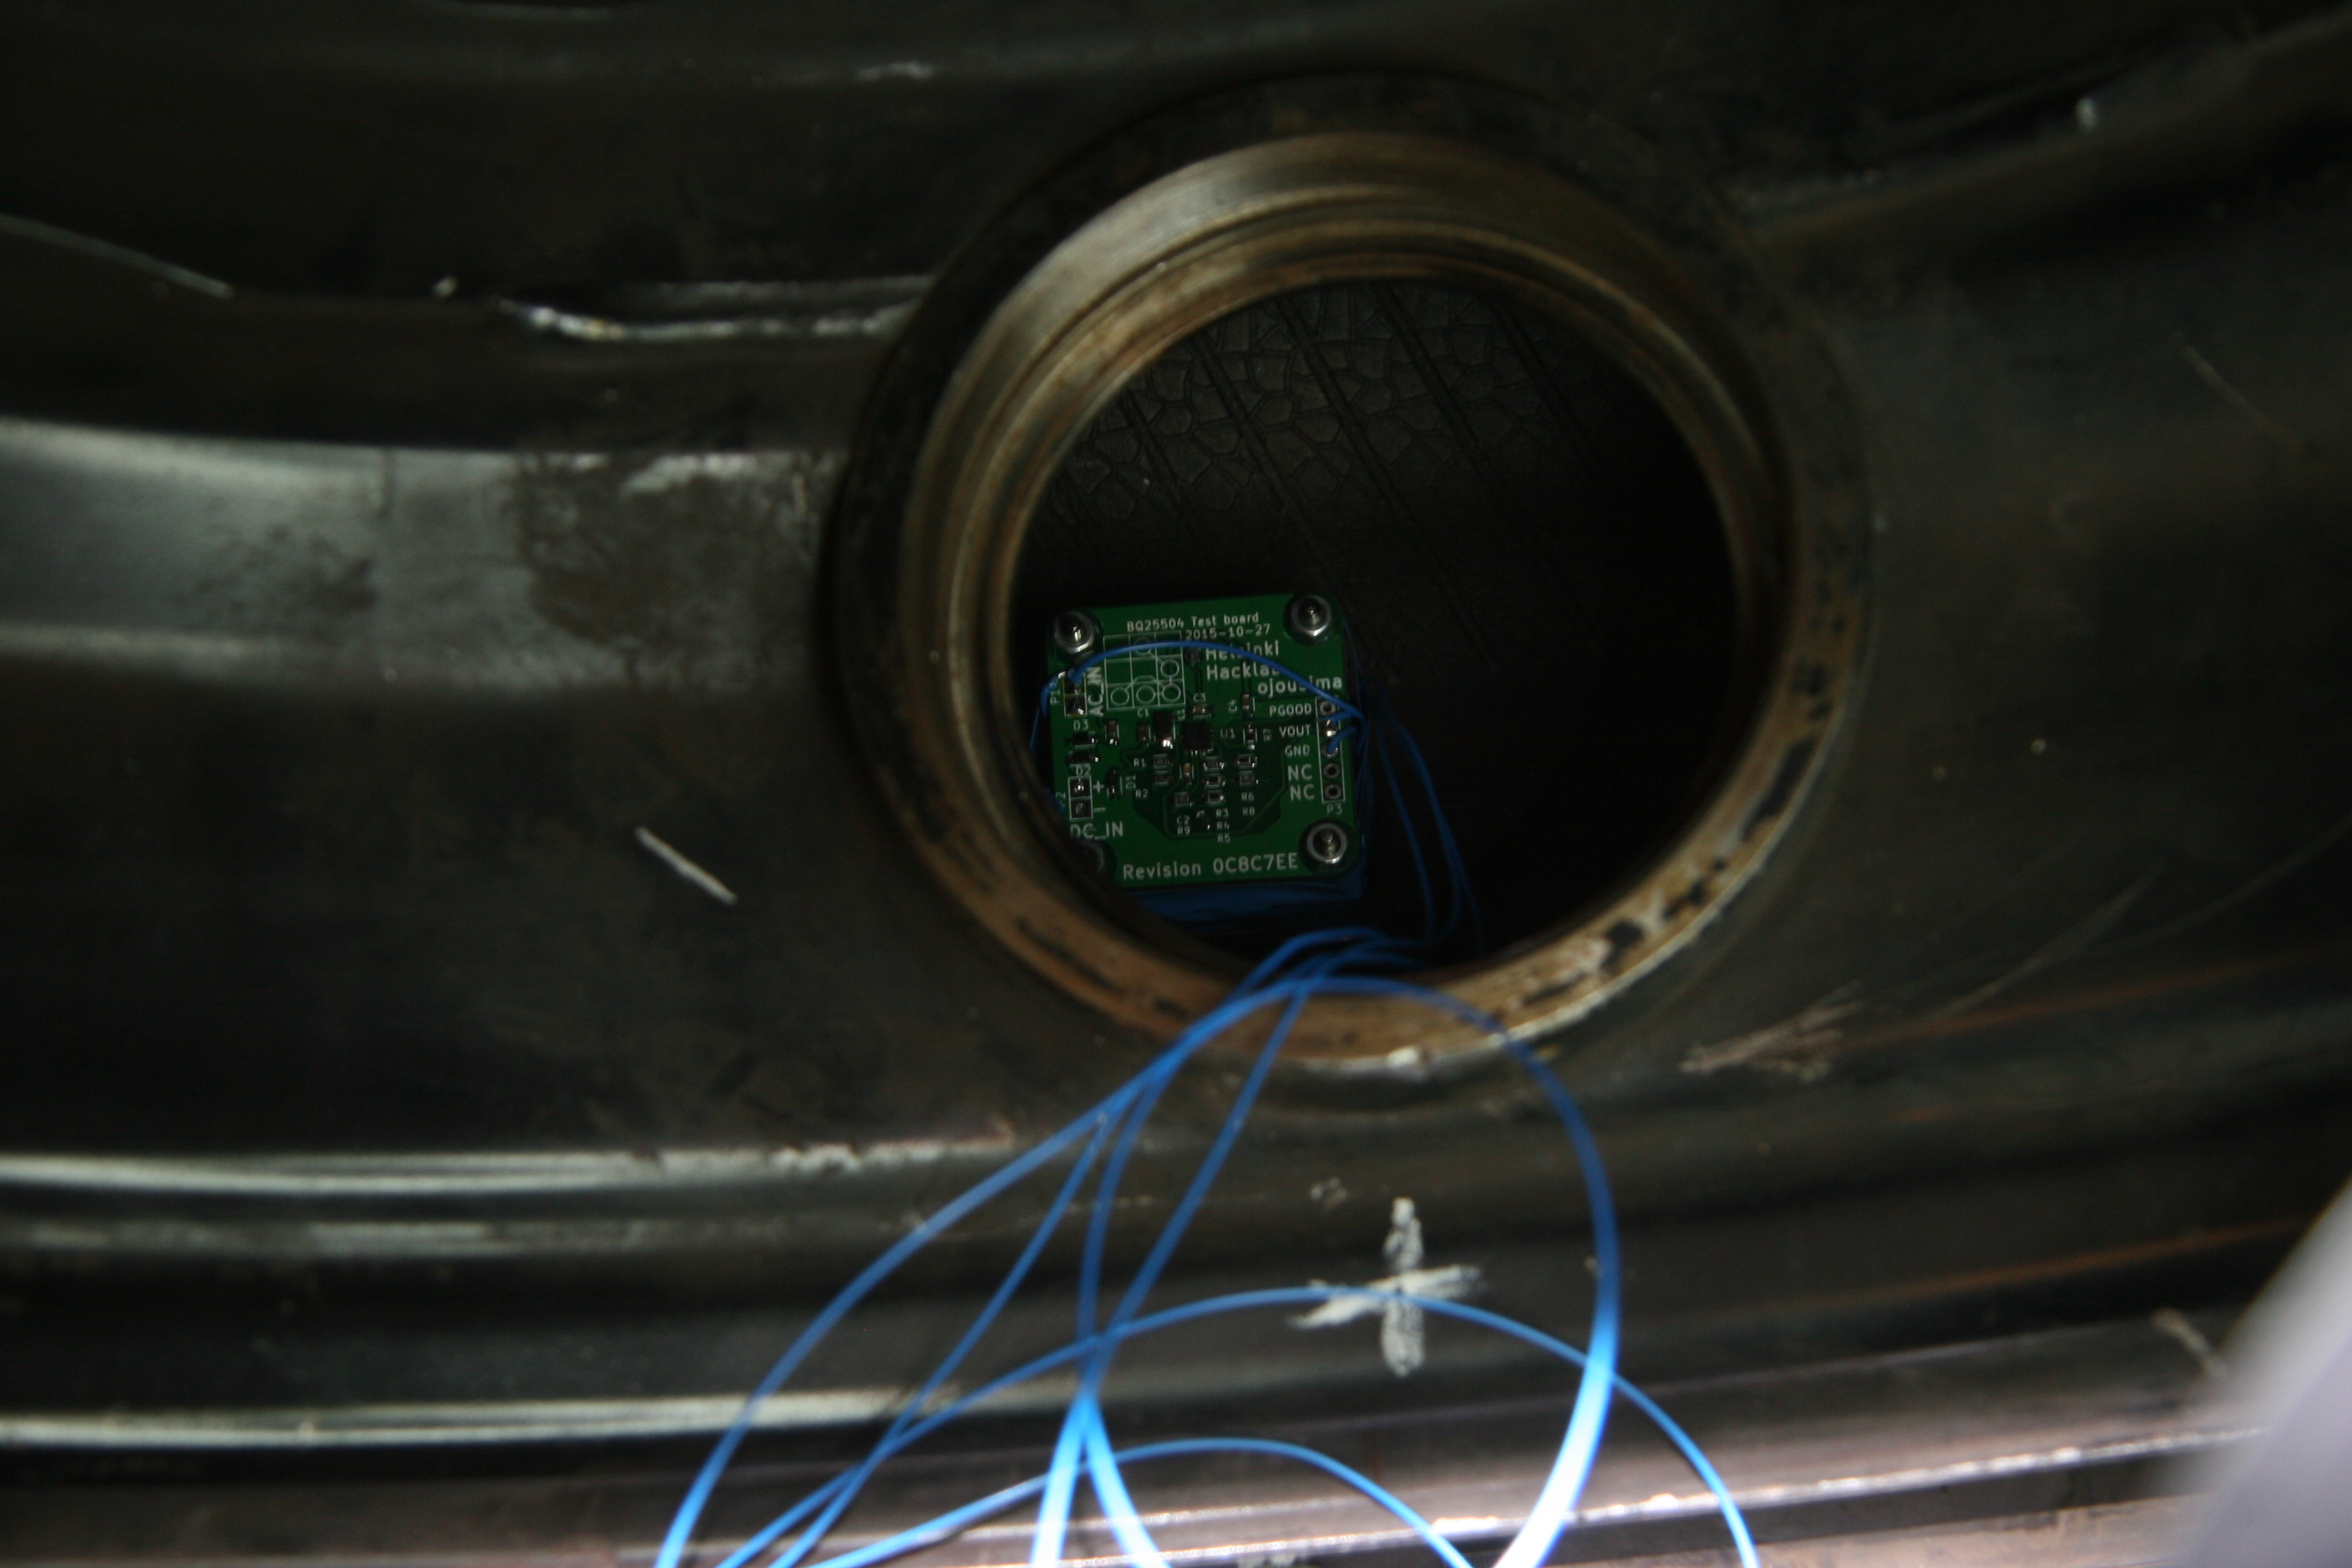
\includegraphics[height=8cm]{images/own_pic/tyre_fixture/piezo_bq_mount.jpg}
\end{center}
\caption{\label{fig:harvester_potted}Piezoelectric harvester mounted inside the tyre.}
\end{figure}

\begin{figure}[htb]
\begin{center}
\includegraphics[height=8cm]{images/own_pic/tyre_fixture/dyno.jpg}
\end{center}
\caption{\label{fig:tyre_platform} Tyre assembled in test platform.}
\end{figure}

The supercapacitor was fully charged before installing in tyre. Measurements were taken next day when the voltage had stabilised near 2.670 V. Tyre was driven at varied speeds and loads. Power output was estimated based stored voltage in supercapacitor before and after the test. The voltage was measured with NI 9215 \cite{ni9215} which has precision required for measuring millivolt-scale differences. 

\begin{table}[htb]
\caption{\label{tbl:piezo_harvester_tyre_output} Measured values from tyre test setup.}
\begin{center}
\fbox{
\begin{tabular}{l l l l l l}
\textbf{Speed} & \textbf{Load} 		& \textbf{V\textsubscript{0}} & \textbf{V\textsubscript{end}} & \textbf{Duration} & \textbf{Power}	  \\ \hline
20 km / h      & 1 kN 		        & 2.674 V        & 2.674 V          & 600 s             & $ 0 \mu W $      	\\ 
20 km / h      & 2 kN 		        & 2.674 V        & 2.676 V          & 600 s             & $ 13 \mu W $      	\\
30 km / h      & 1 kN 		        & 2.676 V        & 2.680 V          & $ \approx $ 300 s     & $ \approx 50 \mu W $       	
\end{tabular}
}
\end{center}
\end{table}

Regrettably the supercapacitor leads to PCB broke down during measurement at 30 km / h and therefore no accurate data was obtained at that speed. However, the results suggest that average power of 50 $\mu$W was obtained from the harvester at 30 km / h speed. The harvesting circuit has a considerable leakage of power at initial charging. This is probably because of the leakage characteristics of the supercapacitor shown in Figure \ref{fig:scap_leakage}. Initial leakage current of a supercapacitor can be in order of tens of microamperes, and it will decrease over course of several days to a specified value \cite{Mars2012}.

\begin{figure}[htb]
\begin{center}
\includegraphics[height=8cm]{images/cited/mars2012.png}
\end{center}
\caption{\label{fig:scap_leakage} Supercapacitors have high initial leakage \cite{Mars2012}.}
\end{figure}

This section presented the real-world power output of piezoelectric harvester. Usable, rectified and regulated power output was at least 13 $\mu W$. Further experiments suggest the energy output is near 50 $\mu W$ at 30 km / h under 2 kN load, . Next section compares the obtained results to current state of art.

\subsection{Comparison to state of art results}\label{sect:state-of-art}
Energy harvesting systems for tyres have been under a lot of research. While there is no standard test process which would give accurately comparable results from different harvester designs, Kubba et al. \cite{Kubba2014} have 
collected a comparison table of various energy harvesting systems for tyres. The results of system designed and built in this work has been appended to results and compared to some similar harvester designs in this section. Table \ref{tbl:results} shows some comparable designs.

\begin{table}[htb]
\caption{\label{tbl:results} The designed system compared to current state of art tyre energy harvester results \cite{Kubba2014}.}
\begin{center}
\fbox{
\begin{tabular}{l l l l l l}
\textbf{Harvester} & \textbf{Size} 		& \textbf{Voltage} & \textbf{Power} & \textbf{Test condition} \\ \hline
Electromagnetic 1      & not specified & 1.5 V AC   & 54 $\mu W$          & 60 km / h \\
Electromagnetic 2      & 10.8 cm\textsuperscript{3} & 200 mV AC   & 400   $\mu W$          & 15 g \\
Electromagnetic 3      & not specified       & 330 mV RMS   & 349   $\mu W$          & 400 rpm \\
Piezoelectric 1        & 0.9 cm\textsuperscript{3} & 6 V AC   & 100   $\mu W$          & Not specified \\
Piezoelectric 2        & 4.1 cm\textsuperscript{3} & 5 V AC   & 47   $\mu W$                   & Not specified \\
Piezoelectric 3        & not specified  & 14 V\textsubscript{p-p} AV & 10   $\mu W$      & Not specified \\ \hline
Piezo presented& 30.6 cm\textsuperscript{3} & not specified & 13   $\mu W$                   & 20 km / h, 2 kN \\
Piezo presented& 30.6 cm\textsuperscript{3} & not specified & 50   $\mu W$ ?                  & 30 km / h, 1 kN 
\end{tabular}
}
\end{center}
\end{table}

The piezoelectric harvester presented in this work produces similar power level as other harvesters in literature. The power output values are not directly comparable as the test setup has been different in each study. However the results obtained in this work can be considered to be in agreement with values presented in literature. 

A typical CR2032 lithium coin cell battery has capacity of approximately 600 mAh at 3 volts. If such a battery were to provide continuously 50 $\mu W$, the battery lifetime would be approximately 4 years. As the energy harvesting system does not produce power continuously, batteries can still provide slightly more power to system over the lifetime of a tyre. If an energy harvesting system could be produced to operate reliably at highway driving speeds, greater amount of power produced might surpass the capacity of battery.
